
% Slideshow, written by Brent Baccala, for a lecture at Catholic University

\documentclass{beamer}
\usetheme{Madrid}

\title{Double Pendulum}
\author{Brent Baccala}
\institute{\tt cosine@freesoft.org}
%% \date{February 8, 2023}

\setbeamertemplate{footline}{}
\beamertemplatenavigationsymbolsempty

\usepackage{xcolor}
\usepackage{comment}
\usepackage{graphicx}

\usepackage{tabularx}

\usepackage{fancyvrb}

\usepackage{tikz}
\usetikzlibrary{angles,quotes}
\usetikzlibrary{calc}

\begin{document}


\begin{frame}
\titlepage
\begin{block}{Abstract}
The Double Pendulum
\end{block}
\end{frame}

\begin{frame}
\begin{exampleblock}{}
\begin{center}
\vskip 20pt
\Huge
Part 1: The Double Pendulum
\vskip 6pt
\ 
\end{center}
\end{exampleblock}
\end{frame}

\begin{frame}
\frametitle{Free Body Diagram}

\begin{tikzpicture}[scale=0.75]

% Define the main coordinates
\coordinate (O) at (0,0);
\coordinate (A) at (3,-4);
\coordinate (B) at (4,-8);

% Draw the pendulum
\draw[thick] (O) -- (A) -- (B);
\draw[dashed] (O) -- +(0,-5);
\draw[dashed] (A) -- +(0,-5);

% Draw the forces
\draw[red,->,thick] (A) -- +(0,-2) node[midway,right] {$m_1g$};
\draw[red,->,thick] (B) -- +(0,-2) node[midway,right] {$m_2g$};
\draw[blue,->,thick] (A) -- (O) node[midway,above] {$T_1$};
\draw[blue,->,thick] (B) -- (A) node[midway,above] {$T_2$};

% Draw the angles
% \draw[->, red, thick] (A) arc (-90:-180:0.75) node {$\theta$};
% \draw[->, red, thick] let \p1 = ($ (A) + (-90:0.75) $) in (A) ++(\p1) arc (-90:-180:0.75) node[midway, below right] {$\theta$};
\draw [->, thick] (O) arc (0:90:2);

% Draw the masses
\fill (A) circle (3pt) node[above left] {$m_1$};
\fill (B) circle (3pt) node[above left] {$m_2$};

\end{tikzpicture}

\end{frame}

\begin{frame}
\frametitle{Energy Calcuation}
\end{frame}

\begin{frame}
\frametitle{Lyapunov Stability}
\end{frame}

\begin{frame}
\frametitle{Double Pendulum Flip Time}
\begin{center}
\vskip -0.1in
\includegraphics[width=0.5\textwidth]{Double_pendulum_flip_time_2021.png}
\end{center}

\tiny
The x and y directions represents the angles that a double pendulum consisting of two uniform bars of same length and mass makes with the vertical direction, being the center of the image 0º and the extremities +- 179.9º. Both bars are initially with zero velocity. The color represents the time (in units of $\sqrt {l/g}$) that it takes for one of the two pendulums to flip, being black less than 1 unit of time, from red to violet it ranges in a logarithm sacel from 1 to 10000 units of time. White means no flip was observed within 10000 units of time.

{\bf Calculation Details:}
The calculations were done using an 8th order Runge-Kutta-Fehlberg embedded with a 7th order method. Tolerance was set to $10^{-10}$ for the maximum absolute value of all four components of the phase space. To give an idea this resulted in an average time step of 0.025 units of time.

{\bf Source:} Wikipedia, {\it Double Pendulum}
%%{\tiny Source: @MathType on Twitter}
%%\includegraphics[clip, trim=0in 2.7in 0in 0in, width=\textwidth]{LU.jpeg}

\end{frame}

\begin{frame}
\frametitle{Effect of Mass Ratio}
\end{frame}

\begin{frame}
\frametitle{Stability of the Solar System}
\end{frame}

\begin{frame}[fragile]
\frametitle{GPT-4 prompt}
\begin{verbatim}
write a sage math script to plot the motion of a
double pendulum with equal point masses and
equal length strings, assuming no friction, no drag

start one pendulum at pi/2 and the other at pi/4

plot the x-y coordinates of both pendulums

be sure to include a shebang line

use matplotlib.pyplot

output only the script without any commentary

\end{verbatim}
\end{frame}

\begin{frame}[fragile]
\frametitle{GPT-4 Makefile}
\begin{Verbatim}[fontsize=\tiny]

# Makefile to call the GPT-4 API to convert a GPT prompt into a sage script to plot a double pendulum.

# We need to use /bin/bash to use pipefail, which is a bash option that causes a pipeline
# to fail if any command in the pipeline fails.  The command in question is "jq", which
# takes the --exit-status option to fail if its output value is null.  That's what I
# want to do if there's some kind of problem (like authentication) with the API call.

SHELL := /bin/bash

URL := https://api.openai.com/v1/chat/completions

pendulum.sage: pendulum.gpt
ifndef OPENAI_API_KEY
	$(error OPENAI_API_KEY is undefined)
endif
	set -o pipefail && jq -n --arg content "$$(cat pendulum.gpt)" \
	  '{ "model": "gpt-4", "messages": [{"role": "user", "content": $$content}], "temperature": 0  }' \
	  | curl $(URL) -H "Content-Type: application/json" -H "Authorization: Bearer $$OPENAI_API_KEY" -d @- \
	  | jq --exit-status -r .choices[0].message.content \
	  | grep -v -e '^```$$' -e '^```python$$' > pendulum.sage
	chmod a+x pendulum.sage
	@cat pendulum.sage
\end{Verbatim}
\end{frame}

\begin{frame}[fragile]
\frametitle{GPT-4 output}
\begin{Verbatim}[fontsize=\tiny]
#!/usr/bin/env sage

import matplotlib.pyplot as plt
import numpy as np
from scipy.integrate import odeint

# Constants
g = 9.81  # gravity
L = 1.0  # length of pendulum
m = 1.0  # mass of pendulum

# Equations of motion
def equations(y0, t):
    theta1, z1, theta2, z2 = y0
    c, s = np.cos(theta1-theta2), np.sin(theta1-theta2)
    theta1_dot = z1
    z1_dot = (m*g*np.sin(theta2)*c - m*s*(L*z1**2*c + L*z2**2) - (2*m)*g*np.sin(theta1)) / L / (2*m - m*s**2)
    theta2_dot = z2
    z2_dot = (2*m)*(L*z1**2*s - g*np.sin(theta2) + g*np.sin(theta1)*c) / L / (2*m - m*s**2)
    return theta1_dot, z1_dot, theta2_dot, z2_dot

# Initial conditions
y0 = np.array([np.pi/2, 0, np.pi/4, 0])

\end{Verbatim}
\end{frame}

\begin{frame}[fragile]
\frametitle{GPT-4 output (cont)}
\begin{Verbatim}[fontsize=\tiny]

# Time array for solution
t = np.linspace(0, 10, 1000)

# Solve ODE
y = odeint(equations, y0, t)

# Extract solutions
theta1, theta2 = y[:,0], y[:,2]

# Convert to Cartesian coordinates
x1 = L * np.sin(theta1)
y1 = -L * np.cos(theta1)
x2 = x1 + L * np.sin(theta2)
y2 = y1 - L * np.cos(theta2)

# Plot
plt.figure()
plt.plot(x1, y1, label='Pendulum 1')
plt.plot(x2, y2, label='Pendulum 2')
plt.legend(loc='best')
plt.xlabel('x')
plt.ylabel('y')
plt.grid()
plt.show()
\end{Verbatim}
\end{frame}

\begin{frame}[fragile]
\frametitle{GPT-4 results}
\vskip -0.4in
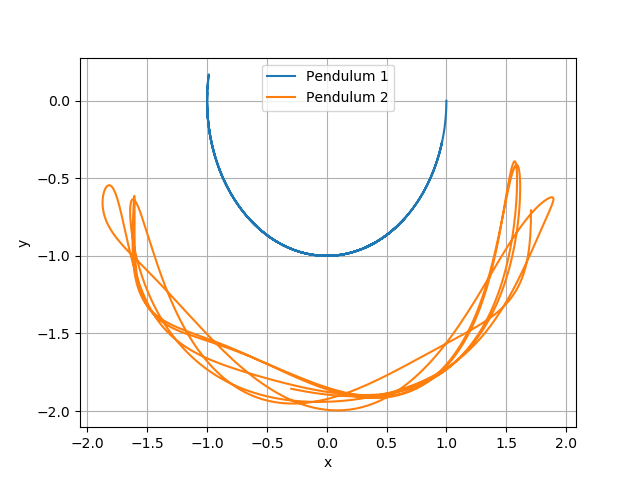
\includegraphics[width=\textwidth]{Figure_1.png}
\end{frame}

\begin{frame}
\begin{exampleblock}{}
\begin{center}
\vskip 20pt
\Huge
Part 2: Use of the Pendulum to Measure Gravity
\vskip 6pt
\ 
\end{center}
\end{exampleblock}
\end{frame}

\begin{frame}
\frametitle{Use of the Pendulum to Measure Gravity}
\begin{itemize}
\item Importance (and difficulty) of Length
\end{itemize}
\end{frame}

\begin{frame}
\frametitle{Piezoelectronics}
\end{frame}

\begin{frame}
\begin{exampleblock}{}
\begin{center}
\vskip 20pt
\Huge
Q: Can a Double Pendulum be used to measure gravity?
\vskip 12pt
If so, how?
\vskip 6pt
\ 
\end{center}
\end{exampleblock}
\end{frame}

\end{document}
